\documentclass[tikz,border=10pt]{standalone}
\usepackage{tikz}
\usetikzlibrary{arrows.meta,calc,positioning,fit,backgrounds}
\usepackage{amsmath,amssymb}
\usepackage{xcolor}
\renewcommand{\familydefault}{\sfdefault}
\pagecolor{white!8}

% ================================================================
% Parameters
% ================================================================

\newcommand{\NInput}{6}
\newcommand{\NEnc}{4}
\newcommand{\NDec}{4}
\newcommand{\NOutput}{6}

\newcommand{\LayerSep}{1.1}

\newcommand{\XInput}{0}
\newcommand{\XEnc}{3.0}
\newcommand{\XLatent}{6.8}
\newcommand{\XZ}{9.8}
\newcommand{\XDec}{12.8}
\newcommand{\XOutput}{15.8}

\newcommand{\NeuronSize}{7.2mm}
\newcommand{\LatentNodeSize}{9mm}

% Colours
\colorlet{encFill}{green!15!white}
\colorlet{encStroke}{green!55!black}
\colorlet{muFill}{orange!15!white}
\colorlet{muStroke}{orange!55!black}
\colorlet{lvFill}{orange!15!white}
\colorlet{lvStroke}{orange!55!black}
\colorlet{zFill}{orange!25!white}
\colorlet{zStroke}{orange!65!black}
\colorlet{decFill}{blue!10!white}
\colorlet{decStroke}{blue!45!black}
\colorlet{wireColor}{black!35}
\colorlet{reparamWire}{black!65}

% ================================================================
% Helpers
% ================================================================

\newcommand{\PlaceLayer}[5]{%
  \pgfmathsetmacro{\half}{(#2-1)/2}%
  \foreach \i in {1,...,#2}{%
    \pgfmathsetmacro{\yy}{(\half-(\i-1))*\LayerSep}%
    \node[circle, draw=#5, line width=0.5pt, minimum size=\NeuronSize,
          inner sep=0pt, fill=#4] (#1\i) at (#3,\yy) {};
  }%
}

\newcommand{\ConnectFull}[4]{%
  \foreach \i in {1,...,#2}{%
    \foreach \j in {1,...,#4}{%
      \draw[wireColor, line width=0.3pt] (#1\i) -- (#3\j);
    }%
  }%
}

% Connect all neurons in a layer to a single target node
\newcommand{\ConnectToOne}[3]{%
  % #1=prefix  #2=count  #3=target node name
  \foreach \i in {1,...,#2}{%
    \draw[wireColor, line width=0.3pt] (#1\i) -- (#3);
  }%
}

% Connect a single source node to all neurons in a layer
\newcommand{\ConnectFromOne}[3]{%
  % #1=source node  #2=prefix  #3=count
  \foreach \i in {1,...,#3}{%
    \draw[wireColor, line width=0.3pt] (#1) -- (#2\i);
  }%
}

\begin{document}
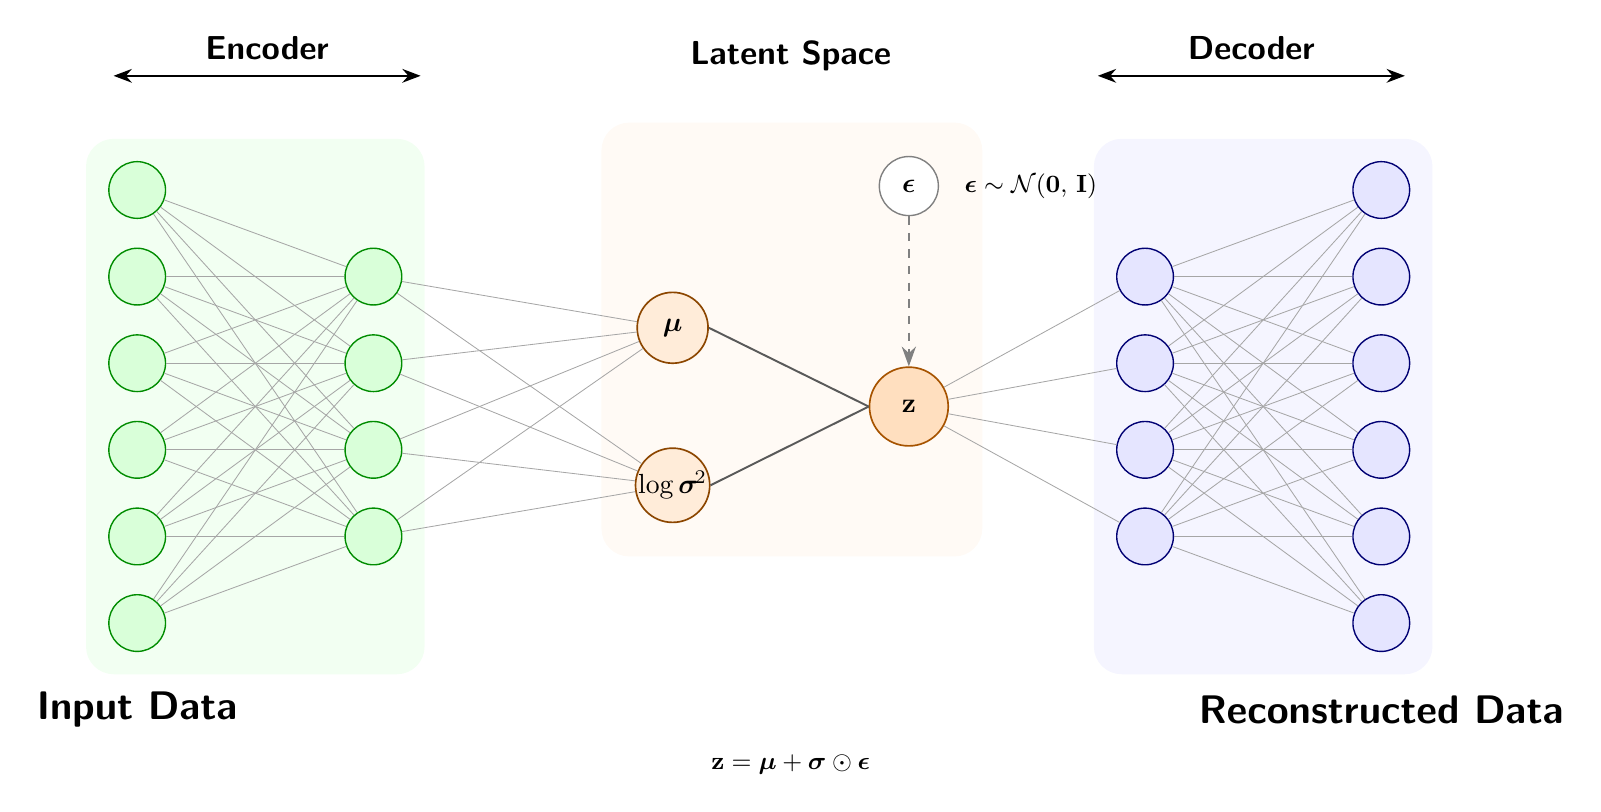
\begin{tikzpicture}[
  >=Stealth,
  title/.style   = {font=\sffamily\bfseries\large},
  biglbl/.style  = {font=\sffamily\bfseries\Large},
  lbl/.style     = {font=\sffamily\bfseries\normalsize},
  note/.style    = {font=\sffamily\small},
  latentnode/.style = {circle, line width=0.6pt, minimum size=\LatentNodeSize,
                       inner sep=0pt, font=\normalsize\bfseries},
  dasharr/.style = {line width=0.8pt, dashed, -{Stealth[length=2.5mm,width=1.8mm]}},
]

% ----------------------------------------------------------------
% Standard neuron layers
% ----------------------------------------------------------------
\PlaceLayer{I}{\NInput}{\XInput}{encFill}{encStroke}
\PlaceLayer{E}{\NEnc}{\XEnc}{encFill}{encStroke}
\PlaceLayer{D}{\NDec}{\XDec}{decFill}{decStroke}
\PlaceLayer{O}{\NOutput}{\XOutput}{decFill}{decStroke}

% ----------------------------------------------------------------
% Latent single nodes — mu above, logvar below, z to the right
% ----------------------------------------------------------------
\node[latentnode, fill=muFill, draw=muStroke]
  (mu) at (\XLatent, 1.0) {$\boldsymbol{\mu}$};

\node[latentnode, fill=lvFill, draw=lvStroke]
  (lv) at (\XLatent, -1.0) {$\log\boldsymbol{\sigma}^{\!2}$};

\node[latentnode, fill=zFill, draw=zStroke, minimum size=10mm]
  (zz) at (\XZ, 0) {$\mathbf{z}$};

% ----------------------------------------------------------------
% Connections
% ----------------------------------------------------------------

% Encoder FC
\ConnectFull{I}{\NInput}{E}{\NEnc}

% Encoder -> mu / logvar  (fan-in to single nodes)
\ConnectToOne{E}{\NEnc}{mu}
\ConnectToOne{E}{\NEnc}{lv}

% mu, logvar -> z  (reparameterization — thicker, darker)
\draw[reparamWire, line width=0.7pt] (mu.east) -- (zz.west);
\draw[reparamWire, line width=0.7pt] (lv.east) -- (zz.west);

% z -> Decoder  (fan-out from single node)
\ConnectFromOne{zz}{D}{\NDec}

% Decoder FC
\ConnectFull{D}{\NDec}{O}{\NOutput}

% ----------------------------------------------------------------
% Noise node (epsilon)
% ----------------------------------------------------------------
\node[circle, draw=black!50, line width=0.5pt, minimum size=7.5mm,
      inner sep=0pt, fill=white, font=\normalsize]
  (eps) at (\XZ, 2.8) {$\boldsymbol{\epsilon}$};

\draw[dasharr, black!50] (eps.south) -- (zz.north);

\node[note, anchor=west] at ($(eps.east)+(0.2,0)$)
  {$\boldsymbol{\epsilon} \sim \mathcal{N}(\mathbf{0},\,\mathbf{I})$};

% ----------------------------------------------------------------
% Section titles
% ----------------------------------------------------------------
\pgfmathsetmacro{\titleY}{4.2}

\draw[<->, line width=0.8pt]
  (\XInput-0.3, \titleY) -- node[above=2pt, title]{Encoder}
  (\XEnc+0.6, \titleY);

\node[title] at ({(\XLatent+\XZ)/2}, \titleY+0.25) {Latent Space};

\draw[<->, line width=0.8pt]
  (\XDec-0.6, \titleY) -- node[above=2pt, title]{Decoder}
  (\XOutput+0.3, \titleY);

% ----------------------------------------------------------------
% Bottom labels
% ----------------------------------------------------------------
\pgfmathsetmacro{\bottomY}{-(\NInput-1)/2*\LayerSep - 1.1}

\node[biglbl] at (\XInput,  \bottomY) {Input Data};
\node[biglbl] at (\XOutput, \bottomY) {Reconstructed Data};

% Reparameterization equation
\node[note] at ({(\XLatent+\XZ)/2}, \bottomY - 0.7)
  {$\mathbf{z} = \boldsymbol{\mu} + \boldsymbol{\sigma} \odot \boldsymbol{\epsilon}$};

% ----------------------------------------------------------------
% Background regions
% ----------------------------------------------------------------
\begin{pgfonlayer}{background}
  \node[rounded corners=10pt, fill=green!5, inner sep=8pt,
        fit=(I1)(I\NInput)(E1)(E\NEnc)] {};
  \node[rounded corners=10pt, fill=orange!4, inner sep=12pt,
        fit=(mu)(lv)(zz)(eps)] {};
  \node[rounded corners=10pt, fill=blue!4, inner sep=8pt,
        fit=(D1)(D\NDec)(O1)(O\NOutput)] {};
\end{pgfonlayer}

\end{tikzpicture}
\end{document}
